\chapter{Worst-Case Execution Time Analysis for Parallel Run-Time Monitoring}
\label{chap:monitoring_wcet}

In order to apply run-time monitoring to traditional real-time systems, we must
be able to analyze the worst-case execution time (WCET) of running a program
with run-time monitoring. The only existing way to do this is to assume that
monitoring is done sequentially. However, this bound is conservative but overly so.

\section{Implicit Path Enumeration}
\label{sec:formulation:ipet}

Most of the WCET analysis techniques today rely on an ILP formulation that is 
obtained from implicit path enumeration techniques \cite{li-ipet-dac95}. 
In this method, a program is converted to a control flow
graph (CFG). From the control flow graph, an ILP problem is formulated that
seeks to maximize
\begin{align*}
  t = \sum_{B \in \mathcal{B}_{CFG}}{N_B \cdot c_{B,max}}
\end{align*} 
where $\mathcal{B}_{CFG}$ is the set of basic blocks in the control flow graph. $N_{B}$
is the number of times block $B$ is executed and $c_{B,max}$ is the maximum number of cycles
to execute block $B$. The maximum value of $t$ is the WCET of the task.  To
account for the fact that only certain paths in the graph will be executed, a
set of constraints are placed on $N_{B}$. For example, on a branch, only one of
the branches will be taken on each execution
of the block. A variable can be assigned to each edge corresponding to the
number of times that edge is taken.
The number of times edges out of the block are taken must equal the number of
times the block is executed.
 Similarly,
the number of times edges into the block are taken must equal the number of
times the block is executed. Various methods have been developed to
create additional constraints to convey other program behavior \cite{li-ipet-dac95, wcetsurvey-tecs08}.
%such as loop
%bounds \cite{li-ipet-dac95} or infeasible paths \cite{suhendra-infeasible-dac09}.

%% Why ILP?
Integer linear programming is an attractive optimization technique
for this problem because the solution found is a global optimum. In
addition, many aspects of program and architecture behavior can be described by
adding constraints to the ILP problem. 
% There have also been several open source
% and commercial ILP solvers written which can be used to find the solution once
% the ILP problem has been formulated. 
Several open source and commercial ILP solvers exist which can solve the formulated ILP problem.
Thus, in developing a method for
estimating the WCET of parallel run-time monitoring, we look to build upon this
ILP framework.

%% Using worst case stalls in original WCET analysis to determine WCET with monitoring.
The IPET-based ILP formulation can be 
extended in a straightforward fashion to incorporate run-time monitoring overheads
if we have the maximum (worst-case) 
%number of cycles that each basic block in the main 
%task spends stalled due to run-time monitoring by maximizing
monitoring stall cycles for each basic block by maximizing
\begin{align*}
  t = \sum_{B \in \mathcal{B}_{CFG}}{N_{B} \cdot (c_{B,max} + s_{B,max})}
\end{align*}
Here, $s_{B,max}$ represents the maximum number of cycles that block $B$ is stalled 
due to monitoring. In this sense, the challenge in WCET analysis with
monitoring lies in determining $s_{B,max}$. 
The rest of this section addresses this problem.

\section{Sequential Monitoring Bound}
\label{sec:formulation:sequential}

One way to determine a conservative bound on the worst-case monitoring stall cycles 
is to consider sequential monitoring.
%rather than parallel monitoring. 
In
sequential monitoring, the monitoring task is run in-line with the main task on the same core
rather than in parallel. That is, after each instruction that would be
forwarded, the monitoring task is run on the main core before the main task
resumes execution. In this case, the WCET estimate can be obtained from 
a traditional method by analyzing one program that contains both main and
monitoring tasks.
The resulting WCET can be considered as a simple bound
for parallel monitoring because it models the case where every forwarded 
instruction causes the main core to stall.
%while the monitoring task is performed. 
However, this bound is
extremely conservative as it does not account for the FIFO buffering or the
parallel execution of the monitoring core. These features are critical to
utilizing run-time monitoring techniques while maintaining low performance
overheads.

% \section{Parameter-Based Method}
% \label{sec:formulation:param}
% 
% % Parameters
% \begin{table}
%   \begin{center}
%     \begin{small}
%     \input{tabs/params}
%     \end{small}
%     \caption{Parameters for parameter-only estimation of worst-case stalls.}
%     \label{tab:formulation.params}
%     \vspace{-0.2in}
%   \end{center}
% \end{table}
% 
% A rough estimate of the worst-case number of cycles stalled can be obtained
% given some parameters describing the main task and the monitoring task. These
% parameters are summarized in Table~\ref{tab:formulation.params}. Suppose that
% the main program has $n_{mon}$ instructions to be monitored. For each monitored
% instruction, the monitoring program has a WCET of $t_{mon}$ to handle the
% instruction. Let the main program's original WCET be $t_{main}$ and the length
% of the FIFO connecting the main and monitoring cores is $n_F$ entries. Given
% only these set of parameters to describe the system, it is unknown whether the
% occurrence of monitored instructions is bursty or sparse. If the monitored
% instructions are sparse then the FIFO can mitigate the amount of cycles
% stalled. However, if the monitored instructions are bursty, then more pressure
% is placed on the FIFO and stalls may increase. Thus, in the worst-case, with
% only these parameters, it must be assumed that all monitored instructions are
% executed consecutively. In this case, it can only be assumed that $n_F + 1$
% monitored instructions do not cause stalls. That is, once the FIFO fills, all
% monitored instructions will cause the main program to stall. An additional
% instruction beyond the FIFO length can be accommodated by being processed by
% the monitoring core and does not need to remain in the FIFO buffers. The amount
% of cycles stalled is then
% \begin{align*}
%   t_{stall} =& (n_{mon} - (l_F + 1)) \cdot t_{mon}
% \end{align*}
% The WCET of the main program with monitoring is then
% \begin{align*}
%   t_{total} =& t_{main} + t_{stall} \\
%   =& t_{main} + (n_{mon} - (l_F + 1))t_{mon}
% \end{align*}
% 
% This estimate is quite conservative because of the assumption that must be made
% that all monitored instructions occur together. By using the program binary, it
% can be determined when monitored instructions occur. However, the assumption
% really stems from the fact that a simple set of parameters cannot fully
% describe the complex interaction of the FIFO with the main and monitoring task.
% A more detailed model of the FIFO needs to be created. 

\section{FIFO Model}
\label{sec:formulation:model}

To obtain tighter WCET bounds, we need to model the FIFO.
The main task can continue its execution as long as a
FIFO entry is available, but needs to stall on a forwarded instruction if
the FIFO is full. The WCET model needs to capture the worst-case (maximum)
number of entries in the FIFO at each forwarded instruction and determine
how many cycles the main task may be stalled due to the FIFO being full. Here,
we propose a mathematical model to express the load in the FIFO and estimate the worst-case stalls.

%In this section, we create a mathematical model to describe the FIFO
%behavior and monitoring stall with respect to the main task. We use similar
%methods as traditional WCET analysis using IPET in order to model the stalls.

In this approach, the original control flow graph must be transformed so that 
each node contains at most one forwarded instruction which is located at the
end of the code sequence represented by the node.
This transformed graph is called a {\em monitoring flow graph (MFG)}.
Intuitively, the analysis needs to consider one forwarded instruction at a time
in order to model the FIFO state on each
forwarded instruction and capture all potential stalls from monitoring. 

To model how full the FIFO is, we define the concept of \emph{monitoring load}.
The monitoring load is the number of cycles required for the monitoring core 
to process all outstanding entries in the FIFO at a given point in time.
The monitoring load increases when a new instruction is 
forwarded by the main task, and decreases as the monitoring core processes
forwarded instructions.  For simplicity, the increase in monitoring load
for any forwarded instruction is conservatively assumed to be the worst-case (maximum) monitoring task
execution time among all possible forwarded instructions. This maximum, $t_{M, max}$, can be obtained from the WCET analysis of the monitoring tasks.
We make this simplification because it is difficult to model the FIFO
mathematically at an entry-by-entry level. With this simplification, each FIFO
entry is identical and so the monitoring load fully represents the state of the FIFO.
% It is difficult to instead model the FIFO mathematically at an
% entry-by-entry level. For example, for two FIFO states with differing entries,
% it is unclear which is the worst-case state without simulating each entry.
The monitoring load cannot be negative and is upper-bounded by the maximum
monitoring load the FIFO can handle, $l_{max}$.  The maximum monitoring load is
the number of FIFO entries, $n_F$, multiplied by the 
% maximum number of cycles
% that the monitoring task can take on one forwarded instruction, $t_{M,max}$,
increase in monitoring load for one forwarded instruction, $t_{M, max}$.
%which can be obtained from the WCET analysis of the monitoring tasks. 

%depending on the number of cycles needed by the
%monitoring task to handle that forwarded instruction. Monitoring load serves as
%a representation of how full the FIFO is. It can also be considered at a given
%point in the main task's code. 

In our context, we need to determine the worst-case (maximum) monitoring load
at the node boundaries in the MFG. 
For a given node, $M$, in the MFG, we define $li_{M}$ as the monitoring load
coming into the node and $lo_{M}$ as the monitoring load exiting the node. The
change in monitoring load for the node is denoted by $\Delta l_{M}$. The maximum
$\Delta l_{M}$ can be calculated as the difference between the WCET of a monitoring
task that corresponds to $M$ and the minimum execution cycles of the node,
$c_{M,min}$: 
\begin{align*}
\Delta l_{M} = 
	\begin{cases}
	t_{M,max} - c_{M,min}, &\text{forwarded inst. } \in M \\
	- c_{M,min}, &\text{no forwarded inst. } \in M
	\end{cases}
\end{align*}
In order to ensure that the analysis is conservative in estimating the worst-case 
(maximum) stalls, we use 
%the worst-case execution time for the monitoring task and 
the best-case (minimum) execution time for the main task here. 
% In particular, we use the worst-case
% processing time for all possible forwarded instructions, $t_{M,max}$, rather than
% a different execution time for each forwarded instruction.
%Here, the worst-case monitoring load for one forwarded instruction 
%l_{max}$, the worst-case cycles to process a forwarded instruction among all
%possible forwarded instructions. 
% This worst-case assumption is needed here
% because we are modeling monitoring load rather than the individual FIFO
% entries.

%The best-case is used here because the
%worst-case cycles of monitoring stalls occur when the time between forwarded
%instructions is minimized. 
%In order to ensure the analysis to be conservative, 
%the monitoring load added for a monitored instruction is assumed to be $\Delta
%l_{max}$, the worst-case cycles to process a forwarded instruction among all
%possible forwarded instructions. This worst-case assumption is needed here
%because we are modeling monitoring load rather than actual FIFO entries. Thus, 

Because the monitoring load is bounded by zero and the maximum load that
the FIFO can handle, $l_{max}$, the monitoring load coming out of a node is
\begin{align*}
	lo_{M} =& 
		\begin{cases}
			0, &li_{M} + \Delta l_{M} < 0 \\
			li_{M} + \Delta l_{M}, &0 \leq li_{M} + \Delta l_{M} \leq l_{max} \\
			l_{max}, &li_{M} + \Delta l_{M} > l_{max}
		\end{cases} \\
  l_{max} =& n_F \cdot t_{M,max}
\end{align*}

The worst-case monitoring load entering node $M$, $li_{M}$, is the largest of the
output monitoring loads among nodes with edges pointing to node $M$. Let
$\mathcal{M_{\text{prev}}}$ represent the set of nodes with edges pointing to node $M$.
Then,
\begin{align*}
	li_{M} = \max_{M_{prev} \in \mathcal{M}_{prev}}lo_{M_{prev}}
\end{align*}

The above equations describe the worst-case monitoring load at each node boundary.
A monitoring stall occurs when a forwarded instruction is executed 
but there is no empty entry in the FIFO buffer. In terms of monitoring
load, if a node would add monitoring load that would cause the resulting total load
to exceed $l_{max}$, then a monitoring stall occurs. The number of cycles
stalled, $s_{M}$, is the number of cycles that this total exceeds $l_{max}$.
% The monitoring stall cycles for node $M$, $m_{M}$, can be obtained from the 
% difference between the unbounded monitoring load, $li_{M} + \Delta l_{M}$ and
% the maximum monitoring load, $l_{max}$. 
That is,
\begin{align*}
	s_{M} =
		\begin{cases}
			0, &li_{M} + \Delta l_{M} < l_{max} \\
			(li_{M} + \Delta l_{M}) - l_{max}, &li_{M} + \Delta l_M \geq l_{max}
		\end{cases}
\end{align*}

%These set of equations describe the monitoring stalls for each node in the MFG,
%using monitoring load as an intermediate variable.
Then, the worst-case monitoring stall cycles for each MFG node can be obtained by maximizing
the sum of the $s_{M}$ across all possible execution paths: 
%can be determined by maximizing the value of each $s_B$.
%This is equivalent to a single objective of maximizing the sum of the $s_B$,
\begin{align*}
  \max \sum_{M \in \mathcal{M}_{MFG}} s_{M}
\end{align*}
where $\mathcal{M}_{MFG}$ is the set of nodes in the MFG.
Once the worst-case stalls for each MFG node is found, the worst-case stalls for
a CFG node, $s_{B,max}$, can be computed by simply summing the stalls from the corresponding MFG 
nodes. We note that since the monitoring
load is always conservative in representing the FIFO state, no timing anomalies
are exhibited by this analysis. That is, determining the individual worst-case
stalls results in the global worst-case stalls.

\section{MILP Formulation}
\label{sec:formulation:milp}

%This objective is linear and so lends itself to LP.  However, several of the
%equations presented in this section for calculating the monitoring load are
%not linear, due to the non-linear behavior of the FIFO. If these equations can
%be converted into linear constraints, then the worst-case monitoring stalls can
%be determined using an LP solver. The following section shows how to convert
%these equations into sets of linear constraints to create a mixed integer
%linear programming problem.

The proposed FIFO model requires solving an optimization problem to obtain the
worst-case stalls, where the input and output monitoring loads, $li_{M}$ and $lo_{M}$, 
and the monitoring stalls, $s_{M}$, need to be determined for each node. Here, we show how
the problem can be formulated using MILP. Although the equations 
for $lo_{M}$ and $s_{M}$ are non-linear, they are piecewise linear. Previous work has
shown that linear constraints for piecewise linear functions can be
formulated using MILP \cite{sierksma-lp}. In the
following constraints, all variables are assumed to be lower bounded by zero
unless otherwise specified, as is typically assumed for MILP.

First, a
set of variables, $lo'$ and $s'$, are created to represent the unbounded
versions of $lo$ and $s$. For readability, the per block subscript $M$ has been
omitted.
% \begin{align*}
% s' =& li + \Delta l - l_{max} \\
% s' >& -\infty \\
% lo' =& li + \Delta l \\
% lo' >& -\infty
% \end{align*}
\begin{align*}
s' =& li + \Delta l - l_{max}, \text{ } s' \in (-\infty, \infty)\\
lo' =& li + \Delta l, \text{ } lo' \in (-\infty, \infty) 
\end{align*}
%Determining $s$ from $s'$ is equivalent to the following piecewise linear
%function.
The following piecewise linear function calculates $s$ from $s'$.
\begin{align*}
s = f(s') = 
  \begin{cases} 
  0, &s' < 0\\
  s', &s' \geq 0
  \end{cases}
\end{align*}
This function can be described in MILP using the following set of constraints.
\begin{align*}
  a_s\lambda_0 + b_s\lambda_2 =& s'\\
  \lambda_0 + \lambda_1 + \lambda_2 =& 1 \\
  \delta_1 + \lambda_2 \leq& 1 \\
  \delta_2 + \lambda_0 \leq& 1 \\
  \delta_1 + \delta_2 =& 1 \\
  b_s\lambda_2 =& s
\end{align*}
where $a_s$ is chosen to be less than the minimum possible value of $s'$ and $b_s$
is chosen to be greater than the maximum possible value of $s'$. The choice of
$a_s$ and $b_s$ is arbitrary as long as it meets these requirements. $\lambda_i$
are continuous variables and $\delta_i$ are binary variables. In this set of
constraints, $s'$ is expressed as a sum of the endpoints of a segment of the 
piecewise function. The $\delta_i$ variables ensure that only the segment
corresponding to $s'$ is considered. $\delta_1 = 1$ corresponds to the $s' < 0$
segment of $f(s')$ and $\delta_2 = 1$ corresponds to the $s' \geq 0$ segment of
$f(s')$. The $\lambda_i$ variables represent exactly where
$s'$ falls on the domain of that segment. $s$ can be calculated using this
information and the values of the function at the segment endpoints.

Similarly, $lo$ can be bound between $0$ and $l_{max}$ by using the following
set of constraints.
\begin{align*}
a_l\lambda_3 + l_{max}\lambda_5 + b_l\lambda_6 =& lo'\\
\lambda_3 + \lambda_4 + \lambda_5 + \lambda_6 =& 1 \\
2 \delta_3 + \lambda_5 + \lambda_6 \leq& 2 \\
2 \delta_4 + \lambda_3 + \lambda_6 \leq& 2 \\
2 \delta_5 + \lambda_3 + \lambda_4 \leq& 2 \\
\delta_3 + \delta_4 + \delta_5 = 1 \\
l_{max}\lambda_5 + l_{max}\lambda_6 =& lo
\end{align*}
As before, $a_l$ and $b_l$ are chosen such that $lo' \in (a_l, b_l)$.
Again, $\lambda_i$ are continuous variables and $\delta_i$  are binary
variables.

Finally, for each node, the input monitoring load $li_{M}$ must be determined.
$li_{M}$ depends on the previous nodes, $\mathcal{M_\text{prev}}$. If there is only
one edge into the node, then $li_M$ is simply
\begin{align*}
li_{M} = lo_{M_{prev}}
\end{align*}
When there is more than one edge into node $M$, one set of constraints is used
to lower bound $li_{M}$ by all $lo_{M_{prev}}$.
\begin{align*}
  li_{M} \geq& lo_{M_{prev}}, \text{ } \forall M_{prev} \in \mathcal{M_\text{prev}}
\end{align*}
Then, another set of constraints upper bounds $li_{M}$ by the maximum $lo_{M_{prev}}$,
\begin{align*}
  li_{M} - b \cdot \delta_{M_{prev}} \leq& lo_{M_{prev}}, \text{ } \forall M_{prev} \in \mathcal{M_\text{prev}} \\
  \sum_{M_{prev} \in \mathcal{M_\text{prev}}}\delta_{M_{prev}} =& |\mathcal{M_\text{prev}}| - 1
\end{align*}
where $b$ is chosen to be greater than $[\max(lo_{M_{prev}}) -\\ \min(lo_{M_{prev}})]$ and
$|\mathcal{M_\text{prev}}|$ is the number of nodes with edges pointing to $M$. $\delta_i$ are binary
variables. The use of the binary variables $\delta_i$ and the second
constraint ensure that $li_{M}$ is only upper bound by one of the $lo_{M_{prev}}$. In
order for all constraints to hold, this must be the maximum $lo_{M_{prev}}$. Together
with the lower bound constraints, these constraints result in $li_{M} =
\max(lo_{M_{prev}})$. For an example of this complete analysis with numbers, see Appendix~\ref{sec:example}.

\vspace{-0.1in}
\section{Evaluation}
\label{sec:evaluation}

% Toolflow
\begin{figure}%[htb]
  \begin{center}
    \vspace{-0.1in}
    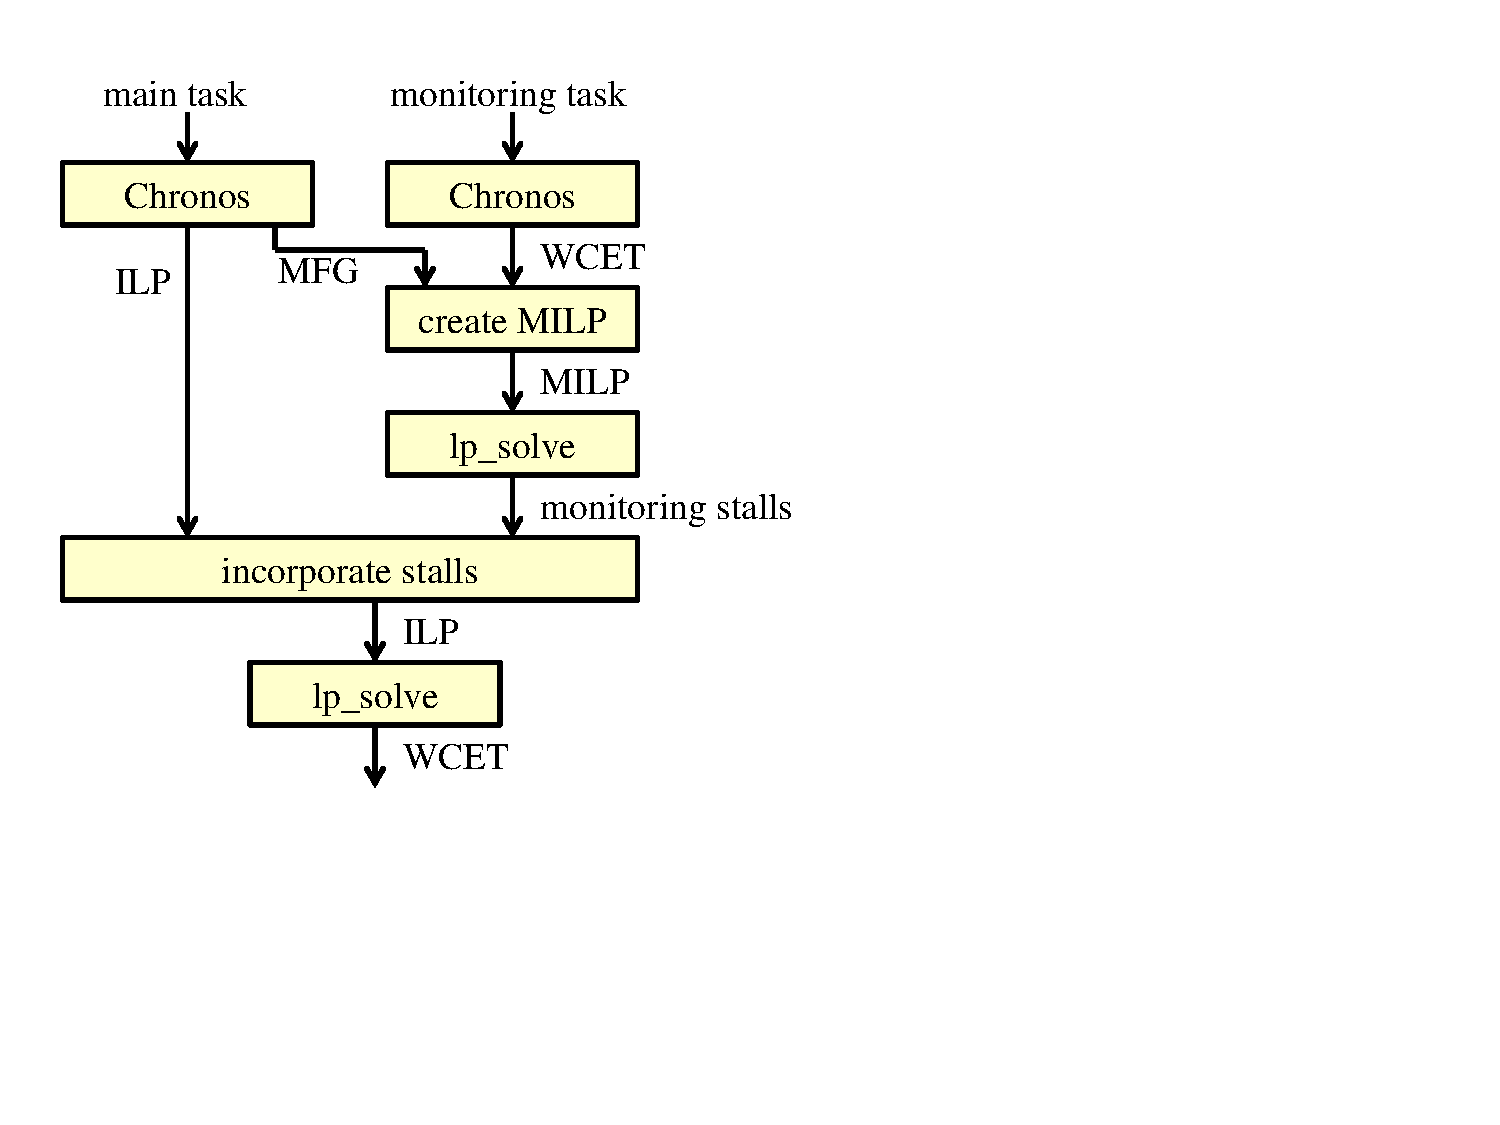
\includegraphics[height=2.2in]{figs/monitoring_wcet/toolflow.pdf}
    \vspace{-0.1in}
    \caption{Toolflow for WCET estimation of parallel monitoring.}
    \label{fig:evaluation.toolflow}
    \vspace{-0.3in}
  \end{center}
\end{figure}

% Results
\begin{table*}[htb]
  \begin{center}
    \begin{small}
    % WCET results 

\begin{tabular}{|l|l||r|r|r|r|r|r|r|}
\hline

\multirow{2}{*}{\bf Monitoring}&\multirow{2}{*}{\bf Experiment}&\multicolumn{7}{c|}{\bf Benchmark}       \\ \cline{3-9}
&&\multicolumn{1}{c|}{\tt cnt}&\multicolumn{1}{c|}{\tt expint}&\multicolumn{1}{c|}{\tt fdct}&\multicolumn{1}{c|}{\tt fibcall}&\multicolumn{1}{c|}{\tt insertsort}&\multicolumn{1}{c|}{\tt matmult}&\multicolumn{1}{c|}{\tt ns} \\ \hline \hline
\multirow{2}{*}{None}&wcet-none&64531&3483&1805&245&598&133668&5951 \\ \cline{2-9}
&sim-none&62931&2293&1805&245&598&133668&5951 \\ \hline \hline
\multirow{3}{*}{UMC}&sequential-umc&103052&3591&4382&257&2489&357453&10338 \\ \cline{2-9}
&wcet-umc&64550&3498&3035&245&2083&256120&5953 \\ \cline{2-9}
&sim-umc&62931&2297&2564&245&1864&235120&5951 \\ \hline \hline
\multirow{3}{*}{CFP}&sequential-cfp&151732&11669&1976&794&1174&231507&18623 \\ \cline{2-9}
&wcet-cfp&93544&8984&1805&547&677&133668&13614 \\ \cline{2-9}
&sim-cfp&72540&5247&1805&382&598&133668&9824 \\ \hline

\end{tabular}

    \end{small}
    \vspace{-0.1in}
    \caption{Estimated and observed WCET (clock cycles) with and without monitoring.}
    \label{tab:evaluation.wcet}
    \vspace{-0.2in}
  \end{center}
\end{table*}

% Calculated ratios
\begin{table*}[htb]
  \begin{center}
    \begin{small}
    % WCET results 

\begin{tabular}{|lll||r|r|r|r|r|r|r||r|r|r|}
\hline

\multicolumn{3}{|c||}{\multirow{2}{*}{\bf Ratio}}  &\multicolumn{7}{c||}{\bf Benchmark}      &\multicolumn{1}{c|}{\multirow{2}{*}{\bf min}}&\multicolumn{1}{c|}{\multirow{2}{*}{\bf max}}&\multicolumn{1}{c|}{\multirow{2}{*}{\bf geomean}} \\ \cline{4-10}
&&&\multicolumn{1}{c|}{\tt cnt}&\multicolumn{1}{c|}{\tt expint}&\multicolumn{1}{c|}{\tt fdct}&\multicolumn{1}{c|}{\tt fibcall}&\multicolumn{1}{c|}{\tt insertsort}&\multicolumn{1}{c|}{\tt matmult}&\multicolumn{1}{c||}{\tt ns}&&& \\ \hline \hline
wcet-none&:&sim-none&1.03&1.52&1.00&1.00&1.00&1.00&1.00&1.00&1.52&1.07 \\ \hline
wcet-umc&:&sim-umc&1.03&1.52&1.18&1.00&1.12&1.09&1.00&1.00&1.52&1.12 \\ \hline
wcet-cfp&:&sim-cfp&1.29&1.71&1.00&1.43&1.13&1.00&1.39&1.00&1.71&1.26 \\ \hline \hline
sequential-umc&:&wcet-umc&1.60&1.03&1.44&1.05&1.19&1.40&1.74&1.03&1.74&1.33 \\ \hline
sequential-cfp&:&wcet-cfp&1.62&1.30&1.09&1.45&1.73&1.73&1.37&1.09&1.73&1.45 \\ \hline \hline
wcet-umc&:&wcet-none&1.00&1.00&1.68&1.00&3.48&1.92&1.00&1.00&3.48&1.41 \\ \hline
wcet-cfp&:&wcet-none&1.45&2.58&1.00&2.23&1.13&1.00&2.29&1.00&2.58&1.55 \\ \hline

\end{tabular}

    \end{small}
    \vspace{-0.1in}
    \caption{Ratios comparing results from different experiments.} \label{tab:evaluation.ratios}
    \vspace{-0.3in}
  \end{center}
\end{table*}

\vspace{-0.0in}
\subsection{Experimental Setup}

Our toolflow for the proposed WCET method is shown in Figure~\ref{fig:evaluation.toolflow}. We
first use Chronos \cite{chronos-tool}, an open source WCET tool, to estimate
the WCET for the main task and the monitoring tasks. We also modified Chronos
to produce a MFG of the main task. This MFG and the monitoring task WCET are used to produce an MILP formulation as in
Section \ref{sec:formulation}. This MILP problem is solved
using lp\_solve \cite{lpsolve}, which produces the worst-case monitoring stall cycles for each forwarded
instruction. These monitoring stalls are combined into the ILP formulation that 
is originally generated for the main task to estimate the overall
WCET with parallel run-time monitoring. Although we use Chronos and lp\_solve
for our implementation, these components can be replaced with any WCET
estimation tool and LP solver respectively.

To evaluate the effectiveness of our WCET scheme, we compared its estimate
with a simple WCET bound from sequential monitoring (Section~\ref{sec:formulation:sequential})
as well as simulation results using the SimpleScalar tool \cite{simplescalar}.
In addition to the WCET estimates with monitoring, we also compared the results with
the WCET of the main task without monitoring, using both Chronos and simulations. 
% The baseline WCET allows us to study the overheads of parallel run-time monitoring
% in terms of the worst-case execution time.

%In order to examine
%how conservative the estimate was, we used the SimpleScalar simulator to
%simulate the benchmarks, both with and without monitoring. 

For the experiments, we configured Chronos and SimpleScalar to model simple processing cores
that execute one instruction per cycle for both main and monitoring cores and used an 8-entry FIFO.
This configuration represents typical embedded microcontrollers, and is designed to focus on 
the impact of parallel run-time monitoring by removing complex features such as branch prediction 
and caches.
%The experiments model an 8-entry FIFO that can buffer up to eight
%forwarded instructions. 
In the evaluation, we used seven benchmarks from the M\"alarden WCET benchmark suite \cite{malarden} 
and two monitoring techniques: uninitialized memory checks (UMC) and control flow protection (CFP).
UMC detects a software bug that reads memory without a write as briefly explained in 
Section~\ref{sec:arch}. CFP protects a program's control flow by checking a target address on
each control transfer \cite{arora-runtime05}. In this technique, a compiler determines a set of valid
targets for each branch and jump in the main task.
This information is stored on the monitoring core. 
On a branch or jump, the monitoring core ensures that the target is
contained in the list of valid targets.


\vspace{-0.05in}
\subsection{Results}

Table~\ref{tab:evaluation.wcet} shows the experimental results for each
benchmark under different configurations. The first set of rows show the WCET 
estimate from Chronos ({\tt wcet-none}) and actual run-times from simulations ({\tt sim-none}) without 
monitoring. The remaining rows show the WCET for the UMC and
CFP monitoring extensions. The results are shown for three different approaches:
a bound from sequential monitoring ({\tt sequential}), our approach ({\tt wcet}),
and simulations ({\tt sim}). The numbers indicate the number of clock cycles.
Appendix~\ref{sec:lptime} includes running times for these experiments.

Table~\ref{tab:evaluation.ratios} shows relative comparisons between
different configurations or WCET methods.
The first set of rows compare the WCET estimates from ILP or MILP formulations
with the worst-case simulation cycles for each monitoring setup. 
The results show that the analytical WCET estimates from our proposed scheme
are larger than the observed WCET by 0\% to 52\% for UMC and 0\% to 71\% for CFP, 
depending on the main task. This difference is comparable to the case without
parallel run-time monitoring, where the analytical WCET from Chronos
is larger than simulation results by 0\% to 52\%. 
In fact, for {\tt expint}, the majority of the difference is from the WCET
estimate of the main task rather than the effects of monitoring.
%In fact, for certain benchmarks, such as {\tt expint}, the majority of the difference 
%is due to estimating the
%WCET of the main task rather than the effects of monitoring. 
This result suggests that our WCET approach is not significantly more conservative than
the baseline WCET tool for the main task.

The second set of rows compare the bound from sequential monitoring and the WCET 
from our proposed method. 
For UMC, our approach shows up to a 74\% reduction in WCET estimates over the simple
bound. Similarly, for CFP, our method shows up to a 73\% improvement.
These results demonstrate that modeling the FIFO decoupling between the main and monitoring
tasks is important for obtaining tight WCET estimates of parallel
monitoring. 

Finally, the last two rows in Table~\ref{tab:evaluation.ratios} compare the WCET 
estimates with and without run-time monitoring.
The results show that the increase in WCET varies significantly depending on
benchmark and monitoring technique. Benchmarks with infrequent monitoring
events (forwarded instructions) show minimal overheads while ones with frequent
monitoring can see significant impacts.
Also, the benchmarks with large WCET increases differ between UMC and CFP.
Therefore, when applying parallel run-time monitoring techniques to real-time systems,
a careful WCET analysis for the given tasks and monitoring techniques 
needs to be performed. 

The impact of run-time monitoring on the execution time in our experiments
(up to 3.48x in UMC and 2.58x in CFP) is roughly in line with previous studies
on multi-cores without any hardware support \cite{chen08-lba, nagarajan08-dift}. 
The performance overheads will be much lower for multi-cores with optimizations 
\cite{chen08-lba} or heterogeneous monitors \cite{flexcore-micro10}. 
Our analysis technique does not depend on any specific monitoring core
microarchitecture and is applicable to more optimized architectures.

%Table~\ref{tab:evaluation.ratios} also compares the WCET estimated with each
%monitoring extension versus the WCET estimated without monitoring. For UMC, the
%WCET is increased by up to 3.48x and for CFP the WCET is increased up to 2.58x.
%However, for both extensions, there also exist benchmarks where the WCET is not
%increased. 

